\documentclass[10pt,a4paper]{article}
\usepackage[UTF8,fontset = windows]{ctex}
\setCJKmainfont[BoldFont=黑体,ItalicFont=楷体]{华文中宋}
\usepackage{amssymb,amsmath,amsfonts,amsthm,mathrsfs,dsfont,graphicx}
\usepackage{ifthen,indentfirst,enumerate,color,titletoc}
\usepackage{tikz}
\usepackage{multicol}
\usepackage{makecell}
\usepackage{longtable}
\usetikzlibrary{arrows,calc,intersections,patterns,decorations.pathreplacing,3d,angles,quotes}
\usepackage[bf,small,indentafter,pagestyles]{titlesec}
\usepackage[top=1in, bottom=1in,left=0.8in,right=0.8in]{geometry}
\renewcommand{\baselinestretch}{1.65}
\newtheorem{defi}{定义~}
\newtheorem{eg}{例~}
\newtheorem{ex}{~}
\newtheorem{rem}{注~}
\newtheorem{thm}{定理~}
\newtheorem{coro}{推论~}
\newtheorem{axiom}{公理~}
\newtheorem{prop}{性质~}
\newcommand{\blank}[1]{\underline{\hbox to #1pt{}}}
\newcommand{\bracket}[1]{(\hbox to #1pt{})}
\newcommand{\onech}[4]{\par\begin{tabular}{p{.9\textwidth}}
A.~#1\\
B.~#2\\
C.~#3\\
D.~#4
\end{tabular}}
\newcommand{\twoch}[4]{\par\begin{tabular}{p{.46\textwidth}p{.46\textwidth}}
A.~#1& B.~#2\\
C.~#3& D.~#4
\end{tabular}}
\newcommand{\vartwoch}[4]{\par\begin{tabular}{p{.46\textwidth}p{.46\textwidth}}
(1)~#1& (2)~#2\\
(3)~#3& (4)~#4
\end{tabular}}
\newcommand{\fourch}[4]{\par\begin{tabular}{p{.23\textwidth}p{.23\textwidth}p{.23\textwidth}p{.23\textwidth}}
A.~#1 &B.~#2& C.~#3& D.~#4
\end{tabular}}
\newcommand{\varfourch}[4]{\par\begin{tabular}{p{.23\textwidth}p{.23\textwidth}p{.23\textwidth}p{.23\textwidth}}
(1)~#1 &(2)~#2& (3)~#3& (4)~#4
\end{tabular}}
\begin{document}
\begin{enumerate}[1.]
\item 求经过下列两点的直线的斜率和倾斜角:\\
(1) $P(-2, 2)$、$Q(2, -2)$;\\
(2) $P(5,\sqrt 3)$、$Q(2,2\sqrt 3)$.
\item 在平面直角坐标系中有一个边长为$1$的正方形$OABC$, 其中$O$为坐标原点, 点$A$、$C$分别在$x$轴和$y$轴上, 点$B$在第一象限. 求直线$OB$和$AC$的斜率.
\item 证明: 在平面直角坐标系中, 如果两条直线平行, 那么它们的倾斜角相等.
\item 求经过点$P(-2,3)$且斜率为$-1$的直线$l$的点斜式方程.
\item 求倾斜角是$\dfrac{5\pi} 6$且在$x$轴上的截距为$-1$的直线$l$的点斜式方程.
\item 求经过点$A(2,3)$且垂直于$x$轴的直线$l$的方程.
\item 已知直线$l$经过点$M(-2,-1)$且在$x$轴、$y$轴上截距相等, 求$l$的方程. 
\item 求经过点$A(-2,3)$、$B(0,6)$的直线$l$的两点式方程.
\item 已知三个不同的点$A(3,1)$、$B(a+1,3)$、$C(2a-1,3-a)$都在一条直线$l$上, 求实数$a$的值和直线$l$的方程.
\item 在平面直角坐标系中, $O$是坐标原点. 已知$A$、$B$两点的坐标分别为$(4,0)$、$
(0,3)$, 分别求$\triangle ABO$的三条边上的中线所在直线的方程. 
\item 求下列方程所表示直线的斜率与倾斜角:\\
(1) $x=1$;\\
(2) $x+y-1=0$;\\
(3) $x+2y-1=0$;\\
(4) $y=1$.
\item 求证: 无论实数$m$取何值, 直线$l:x+(m+1)y+1=0$都经过一个定点.
\item 已知直线$l:kx+2y+3-k=0$经过平面直角坐标系的第二、第三与第四象限, 求实数$k$的取值范围.
\item 写出下列直线的一个法向量:\\
(1) $2x-3y+1=0$;\\
(2) $3x+2y+1=0$;\\
(3) $x+3=0$;\\
(4) $y=\dfrac 12x-3$.
\item 已知直线$l$的方程是$(a-3)x+(2a+1)y-3=0$, 它的一个法向量是$\overrightarrow n=(3,2)$. 求实数$a$的值.
\item 根据下列条件, 求直线$l$的方程:\\
(1) $l$在$x$轴上的截距为$-1$, 且$l$的一个法向量是$\overrightarrow n=(-1,2)$;\\
(2) $l$经过点$(2,3)$, 且$l$上的任何向量都与向量$\overrightarrow a=(1,2)$平行.
\item 判断下列两条直线的位置关系. 若相交, 求交点坐标.\\
(1) $l_1: x+3y+1=0$, $l_2: 3x+4=0$;\\
(2)$ l_1: x-3y+1=0$, $l_2: y=\dfrac 13x+4$.
\item 已知直线$l_1: (a+1)x+y+a=0$, $l_2:x+(a+1)y-2=0$. 若$l_1\parallel l_2$, 求实数$a$的值.
\item 求经过直线$l_1: x-y-4=0$与$l_2:2x-3y-7=0$的交点, 且与直线$l_3: 2x+y+1=0$平行的直线$l$的方程. 
\item 已知直线$l_1:(a-2)x+ay-2=0$与$l_2:(1-a)x+(a+1)y+1=0$互相垂直, 求实数$a$的值.
\item 求过点$(-1,-1)$且分别与下列直线垂直的直线方程:\\
(1) $y=2$;\\
(2) $y=x$;\\
(3) $2x+y+2=0$;\\
(4) $x\cos\theta +y\sin \theta =1$, $\theta$为给定的实数. 
\item 根据下列方程, 求直线$l_1$与$l_2$的夹角的大小:\\
(1) $l_1: 3x-5y+1=0$与$l_2:2x+y=3$;\\
(2) $l_1: y=5x-3$与$l_2:y=-3x+2$.
\item 已知直线$l1:\sqrt 3x-y+3=0$与直线$l_2: y=kx+3$的夹角为$\dfrac \pi 4$, 求实数$k$的值.
\item 求经过点$A(4,-3)$且与直线$l: x+y-3=0$的夹角为$\dfrac\pi 3$的直线$l'$的方程. 
\item 根据下列条件, 求点$M(-2,-1)$到直线$l$的距离$d$:\\
(1) $l: x=3$;\\
(2) $l: y=3$;\\
(3) $l: x+y=3$;\\
(4) $l: y=3x-5$.
\item 在直角三角形$ABC$中, $\angle A=\dfrac \pi 2$, $|AB|=6$, $|AC|=8$. 求三角形的重心$G$到斜边$BC$所在直线的距离. 
\item 求以$C(3,4)$为圆心, 且过点$M(1,-3)$的圆的方程.
\item 求以$C(-1,2)$为圆心, 且与直线$2x-3y-5=0$相切的圆的方程.
\item 一个圆与$y$轴相切于点$(0,4)$, 且在$x$轴正半轴上截得长为$6$的弦. 求此圆的方程. 
\item 求经过$A(3,2)$、$B(1,1)$、$C(2,-1)$三点的圆的方程.
\item 讨论方程$x^2+y^2-2y+\lambda (x^2+y^2-2x)=0$($\lambda$为实数)所表示的曲线.
\item 已知两点$A(-5,0)$、$B(5,0)$, 动点$P$到点$A$的距离是它到点$B$的距离的$3$倍. 求点$P$的轨迹方程. 
\item (1) 求经过点$(-3,4)$且与圆$x^2+y^2=25$相切的直线的方程;\\
(2) 求经过点$(2,4)$且与圆$x^2+y^2=4$相切的直线的方程.
\item 当$a$为何值时, 直线$x+y-a=0$与圆$x^2+y^2=2$分别有如下位置关系:\\
(1) 相交;\\
(2) 相切;\\ 
(3) 相离.
\item 已知直线$l$经过点$P(6,-4)$且被圆$x^2+y^2=20$截得长为$6\sqrt 2$的弦, 求$l$的方程. 
\item 已知圆$C_1:(x-2)^2+(y-2)^2=1$和圆$C2:x^2+(y-m)^2=m^2$($m>0$), 当$m$为何值时, 圆$C_1$与圆$C2$分别内切、相交?
\item 求与圆$x^2+y^2=25$外切于点$P(4,-3)$且半径为$1$的圆的方程.
\item 已知圆$x^2+y^2-2x+2y-3=0$和圆$x^2+y^2+4x-1=0$相交于$A$、$B$两点, 求公共弦$AB$的长.
\item 分别写出满足下列条件的动点$P$的轨迹方程:\\
(1) 点$P$到点$F_1(-3,0)$、$F_2(3,0)$的距离之和为$10$;\\
(2) 点$P$到点$F_1(0,-2)$、$F_2(0,2)$的距离之和为$12$;\\
(3) 点$P$到点$F_1(-4,0)$、$F_2(4,0)$的距离之和为$8$.
\item 分别写出满足下列条件的椭圆的标准方程:\\
(1) 焦点在$y$轴上, 焦距为$2\sqrt {15}$, 且经过点$(0,-4)$;\\
(2) 焦距为$4$, 且经过点$(\sqrt 5,0)$.
\item 已知下列椭圆的方程, 分别求椭圆的长轴长、短轴长、焦点坐标和顶点坐标:\\
(1) $\dfrac{x^2}4+\dfrac{y^2}3=1$;\\
(2) $25x^2+4y^2=100$.
\item 用离心率作为指标衡量, 下列每组两个椭圆中哪一个更接近圆?\\
(1) $\dfrac{x^2}4+\dfrac{y^2}9=1$与$\dfrac{x^2}{16}+\dfrac{y^2}{12}=1$;\\
(2) $x^2+9y^2=36$与$5x^2+3y^2=30$.
\item 若一椭圆以原点为中心, 一个焦点的坐标为$(\sqrt 2,0)$, 且长轴长是短轴长的$\sqrt 3$倍. 求该椭圆的标准方程. 
\item 已知$P$是椭圆$\dfrac{x^2}{36}+\dfrac{y^2}{20}=1$上一个动点, $F_1$是椭圆的左焦点. 求$|PF_1|$的最大值和最小值.
\item 点$P$在焦点为$F_1$、$F_2$的椭圆$\dfrac{x^2}{45}+\dfrac{y^2}{20}=1$上, 且$\angle F_1PF_2=90^\circ$. 求$|PF1|\cdot |PF_2|$的值.
\item 已知直线$l: y=mx-2$与椭圆$C: \dfrac{x^2}4+\dfrac{y^2}3=1$相交于两个不同的点, 求实数$m$的取值范围.
\item 已知$F_1(-5,0)$、$F_2(5,0)$两点, 根据下列条件, 写出动点$M$的轨迹方程:\\
(1) $|MF_1|-|MF_2|=10$;\\
(2) $|MF_1|-|MF_2|=8$;\\
(3) $|MF_1|-|MF_2|=6$.
\item 已知双曲线$\dfrac{x^2}9-\dfrac{y^2}m=1$的焦点在$x$轴上, 焦距为$10$. 求实数$m$的值.
\item 已知双曲线$\dfrac{x^2}{16}-\dfrac{y^2}9=1$的两个焦点分别为$F_1$、$F_2$, $P$为双曲线上一点, 且$\angle F_1PF_2=\dfrac \pi 2$. 求$\triangle PF_1F_2$的面积. 
\item 分别写出下列双曲线的实半轴长、虚半轴长、离心率、焦点坐标、顶点坐标和渐近线方程:\\
(1) $9x^2-16y^2=144$;\\
(2) $\dfrac{y^2}4-\dfrac{x^2}3=1$.
\item 在下列双曲线中, 以$y=\pm \dfrac 12x$为渐近线的是
\bracket{20}.
\fourch{$\dfrac{x^2}{16}-\dfrac{y^2}4=1$}{$\dfrac{x^2}4-\dfrac{y^2}{16}=1$}{$\dfrac{x^2}2-y^2=1$}{$x^2-
\dfrac{y^2}2=1$}
\item 判断双曲线$\dfrac{x^2}4-\dfrac{y^2}5=1$与双曲线$\dfrac{y^2}5-\dfrac{x^2}4=1$的四个焦点是否共圆. 
\item 求适合下列条件的双曲线的标准方程:\\
(1) 顶点在$x$轴上, 两顶点间的距离是$10$, 且经过点$(10,3)$;\\
(2) 一个焦点的坐标为$(5,0)$, 一条渐近线方程为$3x-4y=0$.
\item 给定一对直线$y=\pm\dfrac ba x$($a>0$, $b>0$), 写出所有以这对直线为渐近线的、实轴在$x$轴上的双曲线的方程.
\item 联系双曲线$\dfrac{x^2}{a^2}-\dfrac{y^2}{b^2}=1$($a>0$, $b>0$)的性质, 讨论并叙述双曲线$\dfrac{y^2}{a^2}-\dfrac{x^2}{b^2}=1$($a>0$, $b>0$)的性质(不要求推理过程).
\item 填写下表:
\begin{center}
\begin{tabular}{|p{.1\textwidth}<{\centering}|p{.2\textwidth}<{\centering}|p{.2\textwidth}<{\centering}|p{.2\textwidth}<{\centering}|p{.2\textwidth}<{\centering}|}
\hline
图示 & 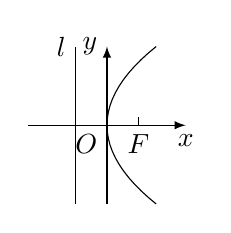
\begin{tikzpicture}[>=latex] 
\draw [->] (-1,0) -- (1,0) node [below] {$x$};
\draw [->] (0,-1) -- (0,1) node [left] {$y$};
\draw (0,0) node [below left] {$O$};
\draw (-0.4,-1) -- (-0.4,1) node [left] {$l$};
\draw (0.4,0.1) -- (0.4,0) node [below] {$F$};
\draw [domain = -1:1] plot ({pow(\x,2)/1.6},\x);
\end{tikzpicture} & 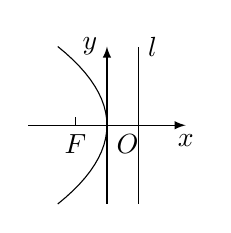
\begin{tikzpicture}[>=latex] 
\draw [->] (-1,0) -- (1,0) node [below] {$x$};
\draw [->] (0,-1) -- (0,1) node [left] {$y$};
\draw (0,0) node [below right] {$O$};
\draw (0.4,-1) -- (0.4,1) node [right] {$l$};
\draw (-0.4,0.1) -- (-0.4,0) node [below] {$F$};
\draw [domain = -1:1] plot ({-pow(\x,2)/1.6},\x);
\end{tikzpicture} &  & \\ \hline
标准方程 & $y^2=2px$($p>0$) & & $x^2=2py$($p>0$) & \\ \hline
焦点坐标 & $(\dfrac p2,0)$ & & & $(0,-\dfrac p2)$ \\ \hline
准线方程 & $x=-\dfrac p2$ & & & $y=\dfrac p2$ \\ \hline
\end{tabular}
\end{center}
\item 分别写出满足下列条件的抛物线的标准方程:\\
(1) 焦点是$F(-2,0)$;\\
(2) 准线方程是$y=1$.
\item 求抛物线$y^2=4x$上到焦点的距离等于$9$的点的坐标.
\item 过点$P(2,4)$且与抛物线$y2=8x$有且只有一个公共点的直线有
\bracket{20}.
\fourch{$1$条}{$2$条}{$3$条}{$4$条}
\item 求抛物线$y^2=4x$上的点到直线$4x+3y+7=0$的最短距离.
\item 由抛物线的标准方程知, 函数$y=\sqrt x$的图像是某条抛物线的一部分. 求这条抛物线的焦点坐标和准线方程.
\item 判断下列各组两个方程是否表示相同的曲线:\\
(1) $y=x$, $\dfrac yx=1$;\\
(2) $y=x$, $y=\sqrt{x^2}$;\\
(3) $|x|=|y|$, $x^2-y^2=0$.
\item 已知$\triangle ABC$的周长为$18$, 且$BC=8$. 建立适当的平面直角坐标系, 求顶点$A$的轨迹方程.
\item 当点$A$在曲线$y=x^2+3$上运动时, 连接点$A$与定点$B(6,0)$. 求$AB$的中点$P$的轨迹方程.
\item 设$a$、$b$是非零常数, 参数方程$\begin{cases} x= a
\cos \alpha, \\ y=b\tan\alpha\end{cases}$($\alpha\ne k\pi +\dfrac \pi 2$, $k\in \mathbf{Z}$)表示的是什么曲线?
\item 以原点为圆心、$1$为半径作一个圆. 设定点$A$的坐标为$(2,0)$, $B$为圆上任意一点, $M$为线段$AB$的中点. 求点$M$轨迹的参数方程.
\item 动点$M$作匀速直线运动, 它在$x$轴和$y$轴方向的分速度分别为$9$和$12$, 运动开始时, 点$M$位于$A(1,1)$. 求点$M$的轨迹的参数方程. 
\item (1) 若约定$\rho>0$, $0\le \theta <2\pi$, 试写出图中$A$、$B$、$C$、$D$、$E$各点的极坐标$(\rho,\theta)$;\\
(2) 若约定$\rho<0$, $0\le\theta <2\pi$, 试写出图中$A$、$B$、$C$、$D$、$E$各点的极坐标$(\rho,\theta)$.
\begin{center}
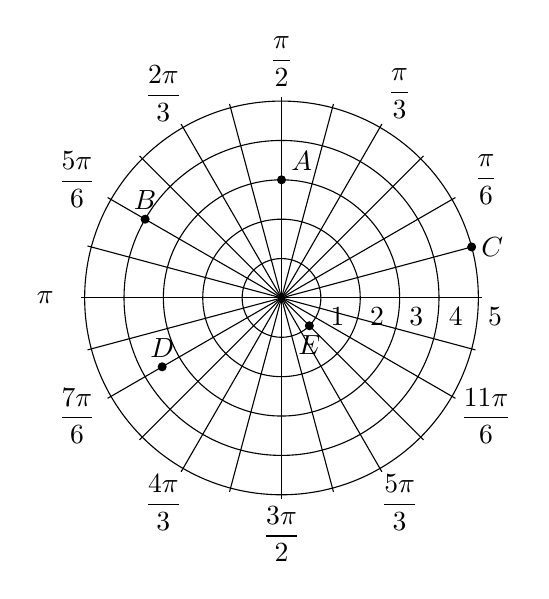
\begin{tikzpicture}[>=latex,scale = 0.5]
\foreach \i in {0,15,...,345} {\draw (0,0) -- (\i:5.1);};
\foreach \i in {1,2,...,5} {\draw (0,0) circle (\i); \draw (\i,0) node [below right] {$\i$};};
\draw (30:6) node {$\dfrac \pi 6$};
\draw (60:6) node {$\dfrac \pi 3$};
\draw (90:6) node {$\dfrac \pi 2$};
\draw (120:6) node {$\dfrac {2\pi} 3$};
\draw (150:6) node {$\dfrac {5\pi} 6$};
\draw (180:6) node {$\pi$};
\draw (210:6) node {$\dfrac {7\pi} 6$};
\draw (240:6) node {$\dfrac {4\pi} 3$};
\draw (270:6) node {$\dfrac {3\pi} 2$};
\draw (300:6) node {$\dfrac {5\pi} 3$};
\draw (330:6) node {$\dfrac {11\pi} 6$};
\filldraw (90:3) circle (0.1) node [above right] {$A$};
\filldraw (150:4) circle (0.1) node [above] {$B$};
\filldraw (15:5) circle (0.1) node [right] {$C$};
\filldraw (210:3.5) circle (0.1) node [above] {$D$};
\filldraw (315:1) circle (0.1) node [below] {$E$};
\end{tikzpicture}
\end{center}
\item 在极坐标系中, 画出点$A(3,\dfrac \pi 4)$、$B(3,-\dfrac \pi 4)$、$C(3,\dfrac{5\pi} 4)$, 并说明$A$和$B$、$C$有怎样的位置关系. 
\item 求经过点$A(a,0)$且和极轴垂直的直线$l$的极坐标方程.
\item (1) 求圆心在极点$O$、半径为$a$的圆的极坐标方程;\\
(2) 求圆心在$(a,\dfrac \pi 2)$、半径为$a$的圆的极坐标方程.
\item 分别画出下列极坐标方程和直角坐标方程的曲线:\\
(1) 极坐标方程$\rho=2$, 直角坐标方程$x=2$;\\
(2) 极坐标方程$\theta=\dfrac \pi 4$, 直角坐标方程$x=\dfrac \pi 4$. 
\item (1) 把点$M$的极坐标$(2,\pi 6)$化成直角坐标;\\
(2) 把点$P$的直角坐标$(-1,\sqrt 3)$化成极坐标.
\item 化直角坐标方程$x^2+y^2-2ay=0$为极坐标方程.
\item 化极坐标方程$\rho=\sin\theta+\cos \theta$为直角坐标方程. 
\item 空间中有异面向量的概念吗? 为什么?
\item 如图, 请在图中找出三个不共面的向量.
\begin{center}
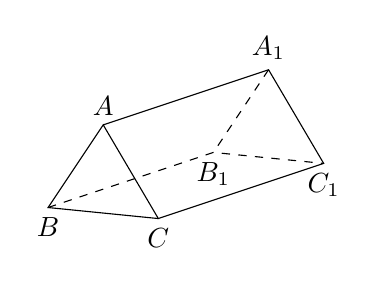
\begin{tikzpicture}[>=latex,scale = 0.7]
\draw (0,0) node [below] {$B$} coordinate (B);
\draw (2,-0.2) node [below] {$C$} coordinate (C);
\draw (1,1.5)  node [above] {$A$} coordinate (A);
\draw (A) ++ (3,1) node [above] {$A_1$} coordinate (A1);
\draw (B) ++ (3,1) node [below] {$B_1$} coordinate (B1);
\draw (C) ++ (3,1) node [below] {$C_1$} coordinate (C1);
\draw (B) -- (C) -- (A) -- cycle (C) -- (C1) -- (A1) -- (A);
\draw [dashed] (B) -- (B1) -- (C1) (A1) -- (B1);
\end{tikzpicture}
\end{center}
\item 化简下列算式:\\
(1) $3(2\overrightarrow a-\overrightarrow b-4\overrightarrow c)-4(\overrightarrow a-2\overrightarrow b+3\overrightarrow c)$;\\
(2) $\overrightarrow{OA}-[\overrightarrow{OB}-(\overrightarrow{AB}-\overrightarrow{AC})]$.
\item 如图, 棱长为$a$的正四面体$ABCD$中, $E$为棱$AB$的中点. 求$\overrightarrow{DC}\cdot \overrightarrow{DE}$与$\overrightarrow{BC}\cdot \overrightarrow{DE}$.
\begin{center}
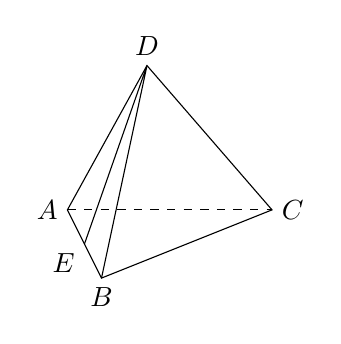
\begin{tikzpicture}[>=latex,scale = 1.5]
\draw ({sqrt(3)/2},0,-0.5) node [right] {$C$} coordinate (C);
\draw ({-sqrt(3)/2},0,-0.5) node [left] {$A$} coordinate (A);
\draw (0,0,1)  node [below] {$B$} coordinate (B);
\draw (0,{sqrt(2)},0)  node [above] {$D$} coordinate (D);
\draw (A) -- (B) -- (C) -- (D) -- cycle;
\draw ($(A)!0.5!(B)$) node [below left] {$E$} -- (D) (B) -- (D);
\draw [dashed] (A) -- (C);
\end{tikzpicture}
\end{center}
\item 设$\overrightarrow a$、$\overrightarrow b$、$\overrightarrow c$是三个空间向量, 求证: $\overrightarrow a\cdot (\overrightarrow b+\overrightarrow c)=\overrightarrow a\cdot \overrightarrow b+
\overrightarrow a\cdot \overrightarrow c$. 
\item 下列命题是否为真命题? 如果是, 请说明理由; 如果不是, 请举出反例.\\
(1) 设$A$、$B$、$C$、$D$是空间中的四个不同的点, 直线$AB$与$CD$是异面直线, 则向量$\overrightarrow{AB}$与$\overrightarrow{CD}$不共面;\\
(2) 如果$\overrightarrow a$、$\overrightarrow b$是平面$\alpha$上的互不平行的向量, 点$C$、$D$不在平面$\alpha$上, 那么向量$\overrightarrow{CD}$与向量$\overrightarrow a$、$\overrightarrow b$不共面;\\
(3) 如果$\overrightarrow a$、$\overrightarrow b$是平面$\alpha$上的互不平行的向量, 点$C$在平面$\alpha$上, 点$D$不在平面$\alpha$上, 那么向量$\overrightarrow{CD}$与向量$\overrightarrow a$、$\overrightarrow b$不共面.
\item 如图, 在长方体$ABCD-A_1B_1C_1D_1$中, $AB:AA_1:AD=
2: 1: 1$, $E$与$F$分别是棱$AB$与$DC$的中点. 设$\overrightarrow{AA_1}=\overrightarrow a,\overrightarrow{AB}=\overrightarrow b$,
$\overrightarrow{AD}=\overrightarrow c$.
\begin{center}
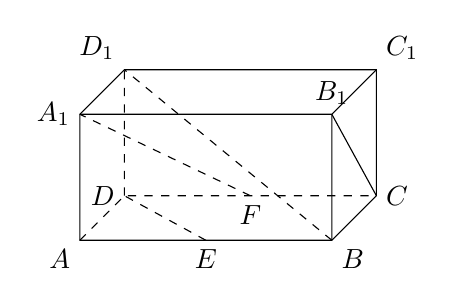
\begin{tikzpicture}[>=latex,scale = 0.8]
\draw (0,0) node [below left] {$A$} coordinate (A) --++ (4,0) node [below right] {$B$} coordinate (B) --++ (45:{2/2}) node [right] {$C$} coordinate (C)
--++ (0,2) node [above right] {$C_1$} coordinate (C1)
--++ (-4,0) node [above left] {$D_1$} coordinate (D1) --++ (225:{2/2}) node [left] {$A_1$} coordinate (A1) -- cycle;
\draw (A) ++ (4,2) node [above] {$B_1$} coordinate (B1) -- (B) (B1) --++ (45:{2/2}) (B1) --++ (-4,0);
\draw [dashed] (A) --++ (45:{2/2}) node [left] {$D$} coordinate (D) --++ (4,0) (D) --++ (0,2);
\draw [dashed] ($(A)!0.5!(B)$) node [below] {$E$} -- (D) ($(C)!0.5!(D)$) node [below] {$F$} -- (A1) (B) -- (D1);
\draw (B1) -- (C);
\end{tikzpicture}
\end{center}
(1) 用向量$\overrightarrow a$、$\overrightarrow b$、$\overrightarrow c$表示$\overrightarrow{BD_1}$、$\overrightarrow{A_1F}$;\\
(2) 求$\overrightarrow{A_1F}\cdot \overrightarrow{B_1C}$;\\
(3) 判断$\overrightarrow{A_1F}$与$\overrightarrow{DE}$是否垂直. 
\item 讨论满足下列条件的点$P$的坐标$(x,y,z)$的特征:
(1) 点$P$在坐标平面上;
(2) 点$P$在坐标轴上.
\item 求向量$\overrightarrow a=(0,1,0)$与$\overrightarrow b=(1,-1,0)$的夹角的大小.
\item 已知向量$\overrightarrow a=(-m,1,3)$平行于向量$\overrightarrow b=(2,n,1)$, 求$m$、$n$.
\item 试证明:\\
(1) 两个平面垂直的充要条件是它们的法向量垂直;\\
(2) 两个平面平行的充要条件是它们的法向量平行.
\item 如图, 在平面$\alpha$与平面$\beta$上分别有不共线的三点$A$、$B$、$C$与$A_1$、$B_1$、$C_1$, 假设$AA_1$、$BB_1$与$CC_1$交于一点$O$, 且$|AO|=|OA_1|$, $|BO|=|OB_1|$, $|CO|=|OC_1|$. 求证: 平面$\alpha\parallel$平面$\beta$.
\begin{center}
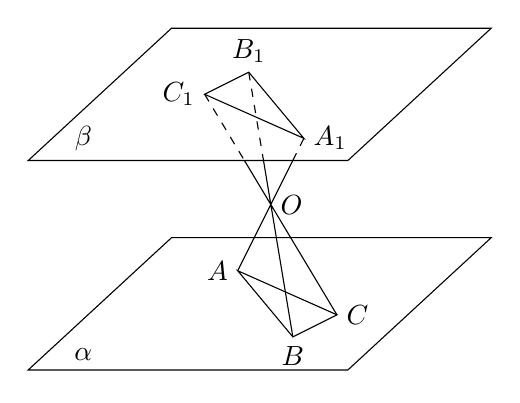
\begin{tikzpicture}[>=latex,scale = 1.4]
\draw (0.4,0.5) --++ (2.9,0) --++ (1.3,1.2) --++ (-2.9,0) -- cycle;
\draw [name path = ceiling] (0.4,0.5) ++ (0,1.9) --++ (2.9,0) --++ (1.3,1.2) --++ (-2.9,0) -- cycle;
\draw (0.9,0.5) node [above] {$\alpha$} (0.9,2.4) node [above] {$\beta$};
\draw (2.6,2) node [right] {$O$} coordinate (O);
\draw (2.3,1.4) node [left] {$A$} coordinate (A);
\draw (2.8,0.8) node [below] {$B$} coordinate (B);
\draw (3.2,1) node [right] {$C$} coordinate (C);
\path [name path = OA] (A) -- ($(A)!2!(O)$) node [right] {$A_1$} coordinate (A1);
\path [name path = OB] (B) -- ($(B)!2!(O)$) node [above] {$B_1$} coordinate (B1);
\path [name path = OC] (C) -- ($(C)!2!(O)$) node [left] {$C_1$} coordinate (C1);
\path [name intersections = {of = OA and ceiling, by = A2}];
\path [name intersections = {of = OB and ceiling, by = B2}];
\path [name intersections = {of = OC and ceiling, by = C2}];
\draw (A) -- (A2) (B) -- (B2) (C) -- (C2);
\draw [dashed] (A1) -- (A2) (B1) -- (B2) (C1) -- (C2);
\draw (A) -- (B) -- (C) -- cycle (A1) -- (B1) -- (C1) -- cycle;
\end{tikzpicture}
\end{center}
\item 如图, $\triangle ABC$中, $AC=BC=\dfrac{\sqrt 2}2AB$, 平面$ABED\perp$平面$ABC$, $ABED$是边长为$1$的正方形, $G$、$F$分别是$EC$、$BD$的中点. 求证:
\begin{center}
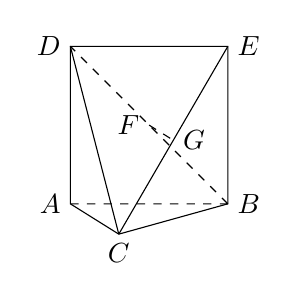
\begin{tikzpicture}[>=latex]
\draw (0,0,0) node [left] {$A$} coordinate (A);
\draw (2,0,0) node [right] {$B$} coordinate (B);
\draw (1,0,1) node [below] {$C$} coordinate (C);
\draw (A) ++ (0,2) node [left] {$D$} coordinate (D);
\draw (B) ++ (0,2) node [right] {$E$} coordinate (E);
\draw (A) -- (C) -- (B) -- (E) -- (D) -- cycle;
\draw (C) -- (D) (C) -- (E);
\draw [dashed] (A) -- (B) (B) -- (D);
\draw [dashed] ($(B)!0.5!(D)$) node [left] {$F$} -- ($(C)!0.5!(E)$) node [right] {$G$};
\end{tikzpicture}
\end{center}
(1) $FG\parallel$平面$ABC$;\\
(2) $AC\perp$平面$EBC$. 
\item 已知三棱锥$ABCD$的三条侧棱$AB$、$AC$、$AD$两两垂直, 且$|AB|=1$, $|AC|=2$, $|AD|=3$. 求顶点$A$到平面$BCD$的距离.
\item 如图, $\triangle ABC$中, $AC=BC=\dfrac{\sqrt 2}2AB$, 平面$ABED\perp$平面$ABC$, $ABED$是边长为$1$的正方形, $G$、$F$分别是$EC$、$BD$的中点, 求直线$FG$与平面$ABC$的距离. 
\begin{center}
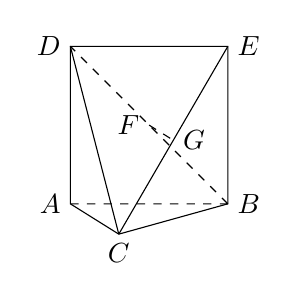
\begin{tikzpicture}[>=latex]
\draw (0,0,0) node [left] {$A$} coordinate (A);
\draw (2,0,0) node [right] {$B$} coordinate (B);
\draw (1,0,1) node [below] {$C$} coordinate (C);
\draw (A) ++ (0,2) node [left] {$D$} coordinate (D);
\draw (B) ++ (0,2) node [right] {$E$} coordinate (E);
\draw (A) -- (C) -- (B) -- (E) -- (D) -- cycle;
\draw (C) -- (D) (C) -- (E);
\draw [dashed] (A) -- (B) (B) -- (D);
\draw [dashed] ($(B)!0.5!(D)$) node [left] {$F$} -- ($(C)!0.5!(E)$) node [right] {$G$};
\end{tikzpicture}
\end{center}
\item 如图, 四边形$ABCD$是矩形, $PA\perp$平面$ABCD$, $E$是线段$PA$的中点. 已知$|PA|=2$, $|AB|=\sqrt 3$, $|BC|=1$. 求异面直线$BE$与$PC$所成角的大小.
\begin{center}
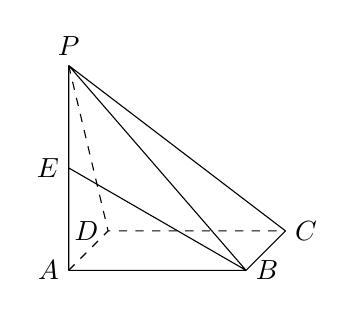
\begin{tikzpicture}[>=latex,scale = 1.3]
\draw (0,0,0) node [left] {$A$} coordinate (A);
\draw ({sqrt(3)},0,0) node [right] {$B$} coordinate (B);
\draw (B) ++ (0,0,-1) node [right] {$C$} coordinate (C);
\draw (A) ++ (0,0,-1) node [left] {$D$} coordinate (D);
\draw (A) ++ (0,2,0) node [above] {$P$} coordinate (P);
\draw ($(A)!0.5!(P)$) node [left] {$E$} coordinate (E);
\draw (P) -- (A) (P) -- (B) (P) -- (C) (A) -- (B) -- (C) (E) -- (B);
\draw [dashed] (A) -- (D) -- (C) (P) -- (D);
\end{tikzpicture}
\end{center}
\item 如图, 在棱长为$1$的正方体$ABCD-A_1B_1C_1D_1$中, $E$是棱$AB$上的动点.
\begin{center}
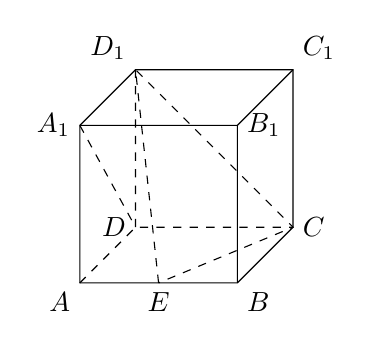
\begin{tikzpicture}[>=latex]
\draw (0,0) node [below left] {$A$} coordinate (A) --++ (2,0) node [below right] {$B$} coordinate (B) --++ (45:{2/2}) node [right] {$C$} coordinate (C)
--++ (0,2) node [above right] {$C_1$} coordinate (C1)
--++ (-2,0) node [above left] {$D_1$} coordinate (D1) --++ (225:{2/2}) node [left] {$A_1$} coordinate (A1) -- cycle;
\draw (A) ++ (2,2) node [right] {$B_1$} coordinate (B1) -- (B) (B1) --++ (45:{2/2}) (B1) --++ (-2,0);
\draw [dashed] (A) --++ (45:{2/2}) node [left] {$D$} coordinate (D) --++ (2,0) (D) --++ (0,2);
\draw ($(A)!0.5!(B)$) node [below] {$E$} coordinate (E);
\draw [dashed] (E) -- (D1) -- (C) -- cycle (A1) -- (D);
\end{tikzpicture}
\end{center}
(1) 求证: $DA_1\perp ED_1$;\\
(2) 确定点$E$的位置, 使得直线$DA_1$与平面$CED_1$所成的角是$45^\circ$. 
\item 在正方体$ABCD-A'B'C'D'$中, $E$、$F$分别是$BC$、$CD$的中点. 求二面角$B-B'E-F$的大小.
\item 如图, 在正方体$ABCD-A_1B_1C_1D_1$中, 求平面$DA_1B$与平面$A_1B_1C_1D_1$所成二面角的正弦值.
\begin{center}
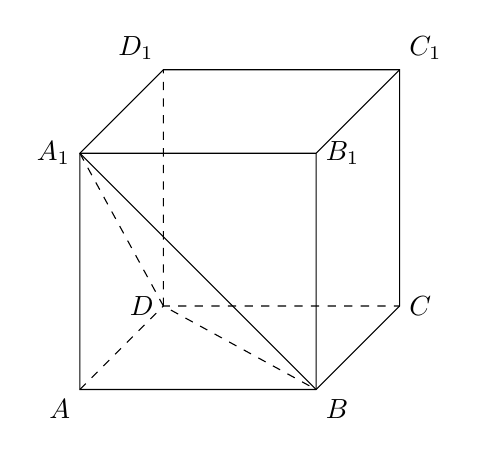
\begin{tikzpicture}[>=latex]
\draw (0,0) node [below left] {$A$} coordinate (A) --++ (3,0) node [below right] {$B$} coordinate (B) --++ (45:{3/2}) node [right] {$C$} coordinate (C)
--++ (0,3) node [above right] {$C_1$} coordinate (C1)
--++ (-3,0) node [above left] {$D_1$} coordinate (D1) --++ (225:{3/2}) node [left] {$A_1$} coordinate (A1) -- cycle;
\draw (A) ++ (3,3) node [right] {$B_1$} coordinate (B1) -- (B) (B1) --++ (45:{3/2}) (B1) --++ (-3,0);
\draw [dashed] (A) --++ (45:{3/2}) node [left] {$D$} coordinate (D) --++ (3,0) (D) --++ (0,3);
\draw (A1) -- (B);
\draw [dashed] (A1) -- (D) -- (B);
\end{tikzpicture}
\end{center}
\item 如图, 在正四棱锥$P-ABCD$中, 底面边长为$2$, 高为$3$. 求二面角$A-PB-C$的大小. 
\begin{center}
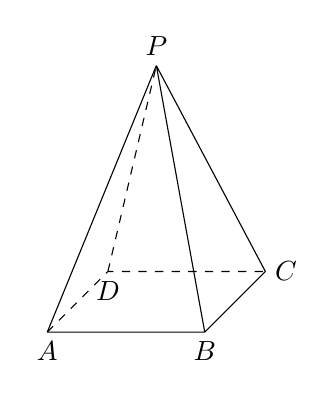
\begin{tikzpicture}[>=latex]
\draw (-1,0,1) node [below] {$A$} coordinate (A);
\draw (1,0,1) node [below] {$B$} coordinate (B);
\draw (1,0,-1) node [right] {$C$} coordinate (C);
\draw (-1,0,-1) node [below] {$D$} coordinate (D);
\draw (0,3,0) node [above] {$P$} coordinate (P);
\draw (P) -- (A) (P) -- (B) (P) -- (C) (A) -- (B) -- (C);
\draw [dashed] (A) -- (D) -- (C) (D) -- (P);
\end{tikzpicture}
\end{center}
\item 下列数列中成等差数列的是\bracket{20}.
\fourch{$0,1,3,5,7$}{$1,\dfrac 13,\dfrac 15,\dfrac 17,\dfrac 19$}
{$1,\sqrt 2,\sqrt 3,2,\sqrt 5$}{$1,\dfrac 13,-\dfrac 13,-1,-\dfrac 53$}
\item 设数列$\{a_n\}$为等差数列, 其公差为$d$.\\
(1) 已知$a_1=-1$, $d=4$, 求$a_8$;\\
(2) 已知$a_7=8$, $d=-13$, 求$a_1$;\\
(3) 已知$a_1=9$, $d=-2$, $a_n=-15$, 求$n$.
\item 已知数列$\{a_n\}$是等差数列, 正整数$m$、$n$、$p$、$q$满足$m+n=p+q$. 求证: $a_m+a_n=a_p+a_q$.
\item 计算$\displaystyle\sum_{i=1}^n 2i$.
\item 设数列$\{a_n\}$为等差数列, 其前$n$项和为$S_n$.\\
(1) 已知$a_1=-4$, $a_8=-18$, 求$S_8$;\\
(2) 已知$a_1=-4$, $a_{12}=18$, 求$S_{15}$.
\item 已知数列$\{a_n\}$的前$n$项和$S_n=n^2-3n$, 求证: 数列$\{a_n\}$是等差数列. 
\item 下列数列中成等比数列的是\bracket{20}.
\fourch{$1,\dfrac 14,\dfrac 19,\dfrac1{16}$}{$1,1,-1,-1$}{$1,\dfrac{\sqrt 2}2,\dfrac 12,\dfrac{\sqrt 2}4$}{$\dfrac 12,2,\dfrac 12,2$}
\item 设数列$\{a_n\}$为等比数列, 其公比为$q$.\\
(1) 已知$a_1=-3$, $q=2$, 求$a_5$;\\
(2) 已知$a_1=1$, $q=2$, $a_n=16$, 求$n$;\\
(3) 已知$a_1=\dfrac 13$, $a_7=9$, 求$q$;\\
(4) 已知$q=-\dfrac 32$, $a_4=-27$, 求$a_1$.
\item 已知数列$\{a_n\}$是等比数列, 正整数$m$、$n$、$s$、$t$满足$m+n=s+t$. 求证: $a_m\cdot a_n=a_s\cdot a_t$. 
\item 设数列$\{a_n\}$为等比数列, 其前$n$项和为$S_n$.\\
(1) 已知$a_1=3$, 公比$q=2$, 求$S_6$;\\
(2) 已知$a_1=-2.7$, 公比$q=-\dfrac 13$, $a_n=\dfrac1{90}$, 求$S_n$.
\item 已知等比数列$\{a_n\}$的前$5$项和为$10$, 前$10$项和为$50$. 求这个数列的前$15$项和.
\item 中国古代数学著作《算法统宗》中有这样一个问题: ``三百七十八里关, 初行健步不为难, 次日脚痛减一半, 六朝才得到其关, 要见次日行里数, 请公仔细算相还.''其意思为: 有一个人要走$378$里路, 第一天健步行走, 从第二天起因为脚痛, 每天走的路程为前一天的一半, 走了$6$天后到达目的地. 请问第二天走了多少里. 
\item 计算$\displaystyle\sum_{i=1}^{\infty}(\dfrac 13)^i$.
\item 化下列循环小数为分数:\\
(1) $0.\dot1 \dot 3$;\\
(2) $1.3\dot 3\dot 2$.
\item 如图, 已知等边三角形$ABC$的面积等于$1$, 连接这个三角形各边的中点得到一个小的三角形$A_1B_1C_1$, 又连接三角形$A_1B_1C_1$各边的中点得到一个更小的三角形$A_2B_2C_2$, 这样的过程可以无限继续下去. 求所有三角形$A_iB_iC_i$($i=1,2,3,\cdots$)的面积的和. 
\begin{center}
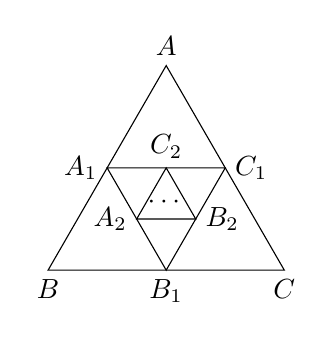
\begin{tikzpicture}[>=latex]
\draw (0,0) node [below] {$B$} coordinate (B) -- (3,0) node [below] {$C$} coordinate (C) --++ (120:3) node [above] {$A$} coordinate (A) -- cycle;
\draw ($(A)!0.5!(B)$) node [left] {$A_1$} coordinate (A1) -- ($(B)!0.5!(C)$) node [below] {$B_1$} coordinate (B1) -- ($(C)!0.5!(A)$) node [right] {$C_1$} coordinate (C1) -- cycle;
\draw ($(A1)!0.5!(B1)$) node [left] {$A_2$} coordinate (A2) -- ($(B1)!0.5!(C1)$) node [right] {$B_2$} coordinate (B2) -- ($(C1)!0.5!(A1)$) node [above] {$C_2$} coordinate (C_2) -- cycle;
\draw (30:{sqrt(3)}) node {$\cdots$};
\end{tikzpicture}
\end{center}
\item 根据数列$\{a_n\}$的通项公式填表:
\begin{center}
\begin{tabular}{|c|c|c|c|c|c|c|c|c|c|}
\hline
$n$ & $1$ & $2$ & $\cdots$ & $5$ & $\cdots$ & $$ & $\cdots$ & $n$ & $\cdots$ \\ \hline
$a_n$ & $$ & $$ & $\cdots$ & $$ & $\cdots$ & $156$ & $\cdots$ & $n(n+1)$ & $\cdots$ \\ \hline
\end{tabular}
\end{center}
\item 图中的三角形图案称为谢宾斯基三角形. 在下图四个三角形图案中, 着色的小三角形的个数依次排列成一个数列的前四项, 请写出其前四项, 并给出这个数列的一个通项公式.
\begin{center}
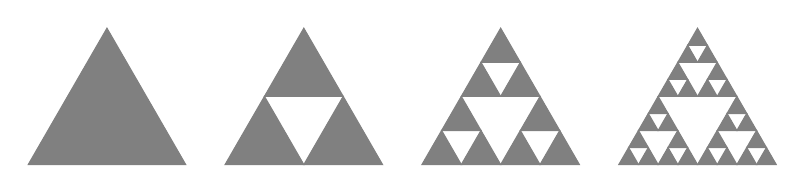
\begin{tikzpicture}[>=latex, gray]
\newcommand{\firstlevel}[2]{\filldraw #1 --++ (#2,0) --++ (120:#2) -- cycle;}
\firstlevel{(0,0)}{2}
\newcommand{\secondlevel}[2]{\firstlevel{#1}{#2/2} \firstlevel{#1 ++ ({#2/2},0)}{#2/2} \firstlevel{#1 ++ (60:{#2/2})}{#2/2}}
\secondlevel{(2.5,0)}{2}
\newcommand{\thirdlevel}[2]{\secondlevel{#1}{#2/2} \secondlevel{#1 ++ ({#2/2},0)}{#2/2} \secondlevel{#1 ++ (60:{#2/2})}{#2/2}}
\thirdlevel{(5,0)}{2}
\newcommand{\fourthlevel}[2]{\thirdlevel{#1}{#2/2} \thirdlevel{#1 ++ ({#2/2},0)}{#2/2} \thirdlevel{#1 ++ (60:{#2/2})}{#2/2}}
\fourthlevel{(7.5,0)}{2}
\end{tikzpicture}
\end{center}
\item 已知数列$\{a_n\}$的通项公式是$a_n=|2n-7|$. 试问: 该数列是否有最小项? 若有, 指出第几项最小; 若没有, 试说明理由. 
\item 已知数列$\{a_n\}$对任意正整数$n$, 均满足$a_1a_2\cdots a_n=n^2$.\\
(1) 写出数列$\{a_n\}$的前五项;\\
(2) 求数列$\{a_n\}$的通项公式.
\item 在数列$\{a_n\}$中, $a_1=2$, 且$a_n=a_{n-1}+\lg\dfrac n{n-1}$($n\ge 2$). 求数列$\{a_n\}$的通项公式.
\item 已知数列$\{a_n\}$满足$a_1=1$, $a_n=2a_{n-1}+3$($n\ge 2$).\\
(1) 求证: 数列$\{a_n+3\}$为等比数列;\\
(2) 求数列$\{a_n\}$的通项公式. 
\item 请指出下列各题用数学归纳法证明过程中的错误.\\
(1) 设$n$为正整数, 求证: $2+4+6+\cdots +2n=n^2+n+1$.\\
证明: 假设当$n=k$($k$为正整数)时等式成立, 即有$2+4+6+\cdots+2k=k^2+k+1$. 那么当$n=k+1$时, 就有$2+4+6+\cdots+2k+2(k+1)
=k^2+k+1+2(k+1)=(k+1)^2+(k+1)+1$. 因此, 对于任意正整数$n$等式都成立.\\
(2) 设$n$为正整数, 求证: $1+2+2^2+\cdots+2^{n-1}=2^n-1$.\\
证明: \textcircled{1} 当$n=1$时, 左边$=1$, 右边$=1$, 等式成立.\\
\textcircled{2} 假设当$n=k$($k$为正整数)时, 等式成立, 即有
$1+2+2^2+\cdots+2^{k-1}=2^k-1$. 那么当$n=k+1$时, 由等比数列求和公式, 就有$1+2+2^2+\cdots+2^{k-1}+2^k=\dfrac{1\times(1-2^{k+1})}{1-2}=2^{k+1}-1$, 等式也成立.\\
根据\textcircled{1}和\textcircled{2}, 由数学归纳法可以断定$1+2+2^2+\cdots+2^{n-1}=2^n-1$对任意正整数$n$都成立.
\item 用数学归纳法证明: $-1+3-5+\cdots+(-1)^n(2n-1)=(-1)^nn$($n$为正整数).
\item 用数学归纳法证明: $1\times 2+2\times 3+3\times 4+\cdots+n(n+1)=\dfrac{n(n+1)(n+2)}3$($n$为正整数). 
\item 已知数列: $\dfrac 1{1\times 2},\dfrac 1{2\times 3},\dfrac 1{3\times 4}, \cdots,\dfrac 1{n(n+1)}, \cdots$, 设$S_n$为该数列的前$n$项和. 计算$S_1,S_2,S_3,S_4$的值; 根据计算的结果, 猜想$S_n$的表达式, 并用数学归纳法加以证明.
\item 已知数列$\{a_n\}$满足$a_1=1$, $a_n+1=\dfrac{3a_n}{a_n+3}$, $a_n\ne 0$.\\
(1) 求$a_2$, $a_3$, $a_4$;\\
(2) 猜想数列$\{a_n\}$的通项公式, 并用数学归纳法加以证明.
\item 是否存在常数$a$、$b$, 使等式$1^2+3^2+5^2+\cdots+(2n-1)^2=an^3+bn$对任意正整数$n$都成立? 证明你的结论. 
\item 在计算$\sqrt 2$的巴比伦算法中, 若选取初值$x_1=-2$, 通过计算器操作, 写出迭代序列的前$5$项.
\item 选取初值$x_1=-2$, 利用递推公式$x_{n+1}=1+ \dfrac1{
x_n+1}$, 通过计算器操作, 写出迭代序列的前$8$项.
\item 仿照计算$\sqrt 2$的巴比伦算法, 构造计算$\sqrt 3$的迭代算法的递推公式, 并选取初值$x_1=1$, 通过计算器操作, 列出该迭代序列的前$5$项. 
\end{enumerate}

\end{document}